%Fiquemos com Deus e Nossa Senhora!
%Sao Jose de Cupertino rogai por nos!!
% ### Uses XeLaTeX ### %
% ### Needs beamer-master ### %
\documentclass[aspectratio=169]{beamer} %. Aspect Ratio 16:9

\usetheme{AI2} % beamerthemeSprace.sty
\usepackage[portuguese]{babel}
\usepackage[utf8]{inputenc}
\usepackage[T1]{fontenc}
\usepackage{ragged2e,gensymb}

\DeclareMathOperator*{\argmin}{arg\,min}
\DeclareMathOperator*{\argmax}{arg\,max}

% DATA FOR FOOTER
\date{2021}
\title{- Máquinas de Vetores de Suporte}
\author{João Paulo Papa}
\institute{Advanced Institute for Artificial Intelligence (AI2)}

\begin{document}
% ####################################
% FIRST SLIDE 						:: \SliTit{This is the Title of the Talk}{A. B. Name}{Sprace}
% SUB-TITLE SLIDE 					:: \SliSubTit{<title>}{<explanation}
% SUB-SUB-TITLE SLIDE				:: \SliSubSubTit{<title>}{<explanation}
% SLIDE WITH TITLE 					:: \SliT{Title}{Content}
% SLIDE NO TITLE 						:: \Sli{Content} 
% SLIDE DOUBLE COLUMN WITH TITLE 	:: \SliDT{Title}{First Column}{Second Column}
% SLIDE DOUBLE COLUMN NO TITLE 		:: \SliD{First Column}{Second Column}
% SLIDE ADVANCED WITH TITLE 			:: \SliAdvT{Title}{Content}
% SLIDE ADVANCED NO TITLE 			:: \SliAdv{Content}
% SLIDE ADVANCED DOUBLE WITH TITLE 	:: \SliAdvDT{Title}{First Column}{Second Column}
% SLIDE ADVANCED DOUBLE NO TITLE 	:: \SliAdvD{First Column}{Second Column}
% SLIDE BLACK						:: \Black{ <Content> }
% SLIDE WHITE						:: \White{ <Content> }
% ITEMIZATION 						:: \begin{itemize}  \iOn{First} \iTw {Second} \iTh{Third} \end{itemize}
% COMMENT TEXT				 		:: \note{<comment>}
% SECTION 							:: \secx{Section} | \secxx{Sub-Section}
% BOLD SPRACE COLOR				:: \bfs{<text>}
% TABLE OF CONTENT					:: \tocitem{<title>}{<content>}
% LEFT ALIGN EQUATION				:: \begin{flalign*}  & <equation> &   \end{flalign*}
% CENTER ALIGN EQUATION	S			:: \begin{gather*} <equations>  \end{gather*}
% SLASH								:: \slashed{<>}
% BAR								:: \barr{<letter>} instead of \bar{<letter>}
% THEREFORE						:: use \portanto (larger and bold}
% 2 or 3 MATH SYMBOLS				:: \overset{<up>}{<down>} &  \underset{<below>}{\overset{<above>}{<middle>}}  
% INSERT TEXT IN FORMULA			:: \ins{<text>}
% EXERCISE							:: \exe{<exercise #>}{<exercise text>}
% SUGGESTED READING BOX			:: \sug{<references>}
% CITATION							:: \cittex{<citation>}
% CITATION DOUBLE COLUMN 			:: \cittexD{<citation>}
% TEXT POSITION						:: \texpos{<Xcm>}{<Ycm>}{<text>} origin = center of slide : x right | y down
% REFERENCE AT BOTTOM  S/D SLIDE		:: \refbotS{<reference>} \refbotD{<reference>}
% HIDDEN SLIDE						:: \hid
% COLOR BOX 						:: \blu{blue} + \red{rec} + \yel{yellow} + \gre{green} + \bege{beige}
% FRAME 							:: \fra{sprace} \frab{blue} \frar{red} + \fray{yellow} + \frag{green}		
% FIGURE 							:: \img{X}{Y}{<scale>}{Figure.png} 
% FIGURE							:: \includegraphics[scale=<scale>]{Figures/.png}
% FIGURE DOUBLE SLIDE NO TITLE		::  \img{-4}{0.5}{<scale>}{Figure.png} % Image 1st half
%									::  \img{4}{0.5}{<scale>}{Figure.png} % Image 2nd half
% FIGURE DOUBLE SLIDE WITH TITLE		::  \img{-4}{0}{<scale>}{Figure.png} % Image 1st half
%									::  \img{4}{0}{<scale>}{Figure.png} % Image 2nd half
% INCLUDING SWF (Flash)				:: \usepackage{media9} and \includemedia >> USE ACROBAT <<
%%%%%%%%%%%%%%%%%%%%%%%%%%%%%%%%%%%%%%%%%%%%%%%%%%
% ###############################################################################
% FIRST SLIDE
\SliTit{{\LARGE Máquinas de Vetores de Suporte}}{Advanced Institute for Artificial Intelligence -- AI2}{https://advancedinstitute.ai}
%%%%%%%%%%%%%%%%%%%%%%%%%%%%%%%%%%%%%%%%%%%%%%%%%%
% ###############################################################################
% SLIDE SUB-TITLE
%\SliSubTit{Sub-Title}{Description}{}
%%%%%%%%%%%%%%%%%%%%%%%%%%%%%%%%%%%%%%%%%%%%%%%%%%
% ###############################################################################
%\SliSubSubTit{Sub-Sub-Title}{Description}
 %%%%%%%%%%%%%%%%%%%%%%%%%%%%%%%%%%%%%%%%%%%%%%%%%%


\SliT{Introdução}{

\justifying As Máquinas de Vetores de Suporte, do inglês \emph{Support Vector Machines} (SVM) são baseadas em conceitos da Teoria do Aprendizado Estatístico (TAE), desenvolvida por Vapnik e colegas. Basicamente, a ideia seria estudar garantias teóricas sobre condições necessárias para o processo de aprendizado.

\justifying Como dito anteriormente, temos duas principais limitações durante um processo de aprendizagem:

\begin{itemize}
	\item supertreinamento (\emph{overfitting}): baixa capacidade de generalização no conjunto de teste.
	\item subtreinamento (\emph{underfitting}): baixa capacidade de aprendizado no conjunto de treinamento.
\end{itemize}
}

\Sli{
\justifying Qual seria a situação ideal? Um \textbf{compromisso} entre as duas situações, ou seja, uma relação custo-benefício entre supertreinamento e subtreinamento. 

\justifying \underline{Definição do problema}: dado um espaço de funções ${\cal F}$, como escolher uma função $\hat{f}\in{\cal F}$ de tal forma que o erro no treinamento seja baixo e a capacidade de generalização seja alta? A TAE nos fornece condições para atingir este objetivo sem assumir uma formulação específica para a distribuição dos dados (abordagem não paramétrica).

\justifying \underline{Objetivo}: Encontrar o melhor classificador $f^\ast\in{\cal F}$ para um conjunto de treinamento fixo com tamanho $m$ de tal forma que se aproxime, ao máximo, do classificador de menor risco, ou seja, $f_{bayes}$.
}

\Sli{
\justifying Quando o aprendizado é \textbf{consistente}, ou seja, quando $f^\ast$ consegue aprender dos dados? Primeiramente, precisamos definir o espaço de funções ${\cal F}$ que o nosso classificador fará parte. Vamos analisar a figura abaixo.

\begin{minipage}{0.43\textwidth}
\begin{center}
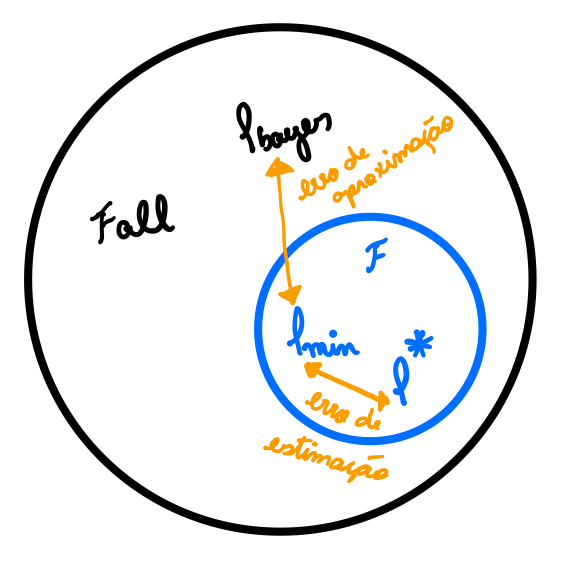
\includegraphics[scale=0.21]{./figs/SVM_Fig1.png}
\end{center}
\end{minipage}%%% to prevent a space
\begin{minipage}{0.49\textwidth}
\begin{itemize}
	\item ${\cal F}_{all}$: espaço de todas as funções possíveis
	\item ${\cal F}$: espaço das funções que o classificador pode aprender
	\item $f_{bayes}$: classificador de mínimo risco possível
	\item $f_{min}$: classificador de mínimo risco em ${\cal F}$
\end{itemize}
\null
\par\xdef\tpd{\the\prevdepth}
\end{minipage}
}

\Sli{
\justify Podemos, então, associar um \textbf{risco} $R$ à cada classificador. Desta forma, $R(f^\ast)$ corresponde ao risco associado ao classificador $f^\ast$.

\justify Temos que um classificador é dito ser \textbf{consistente} se, e somente se, o seu risco é minimizado quando $m\rightarrow\infty$, ou seja, quando o conjunto de treinamento aumenta. Em outras palavras, a consistência nos diz se estamos conseguindo aprender ou não.

\justify O grande problema é que, quando ${\cal F}\rightarrow{\cal F}_{all}$, o nosso aprendizado não é consistente, pois o espaço de funções possíveis aumenta muito. Assim, devemos restringir o tamanho de ${\cal F}$. No entanto, o nosso dilema é: \textbf{ao restringirmos ${\cal F}$, o nosso erro de aproximação fica grande; ao ampliarmos ${\cal F}$, o nosso erro de estimação aumenta.}
}

\Sli{
\justify A pergunta principal é: \textbf{como escolher ${\cal F}\subset{\cal F}_{all}$ e $f^\ast\in{\cal F}$?} A TAE nos ajuda a responder à essa questão propondo as SVMs, que é uma classe de (funções) classificadores ótimas no que diz respeito ao \textbf{compromisso} entre os erros de aproximação e estimação.

\justify \underline{Objetivo}: encontrar um hiperplano que maximize a \textbf{margem} de segurança e cometa poucos \textbf{erros marginais}, isto é, minimize o risco. O que são erros marginais?

\begin{center}
\begin{tabular}{cc}
	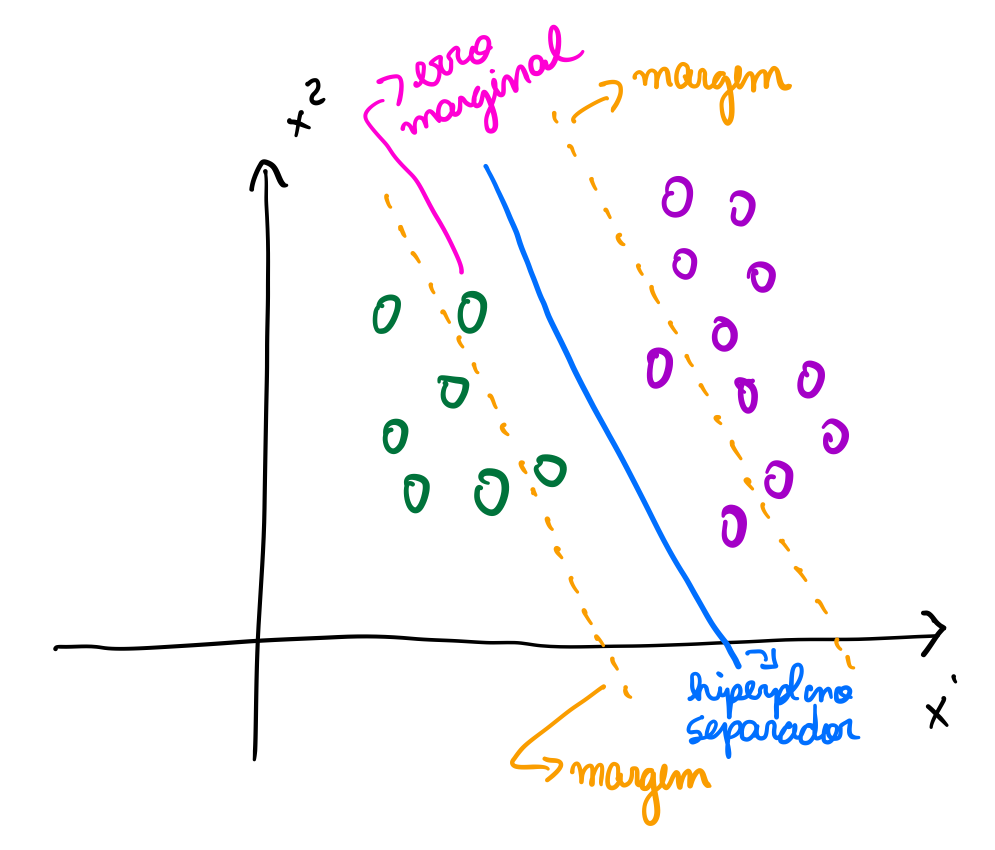
\includegraphics[scale=0.15]{./figs/SVM_Fig2.png} &\hspace{2cm}
	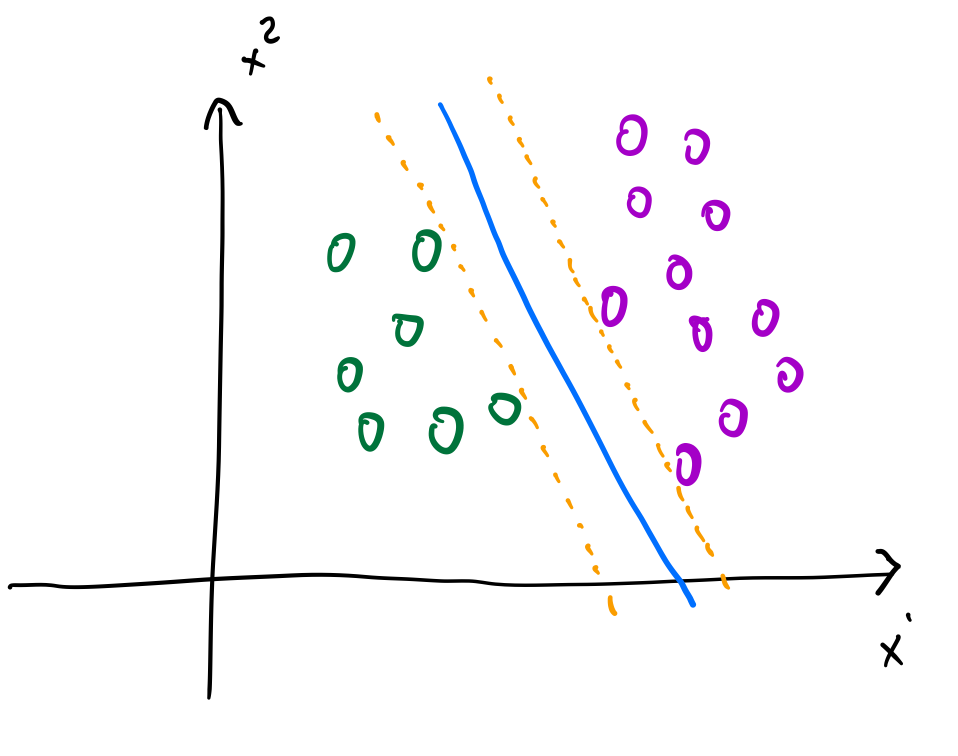
\includegraphics[scale=0.15]{./figs/SVM_Fig3.png}
\end{tabular}
\end{center}
}

\Sli{
\justify Fazemos uma analogia com o algoritmo do Perceptron no sentido que ambos utilizam uma função de decisão linear, ou seja, um hiperplano. A diferença é que o hiperplano do Perceptron não possui as \textbf{propriedades ótimas} que o hiperplano encontrado pelo SVM possui.

\begin{center}
\begin{tabular}{cc}
	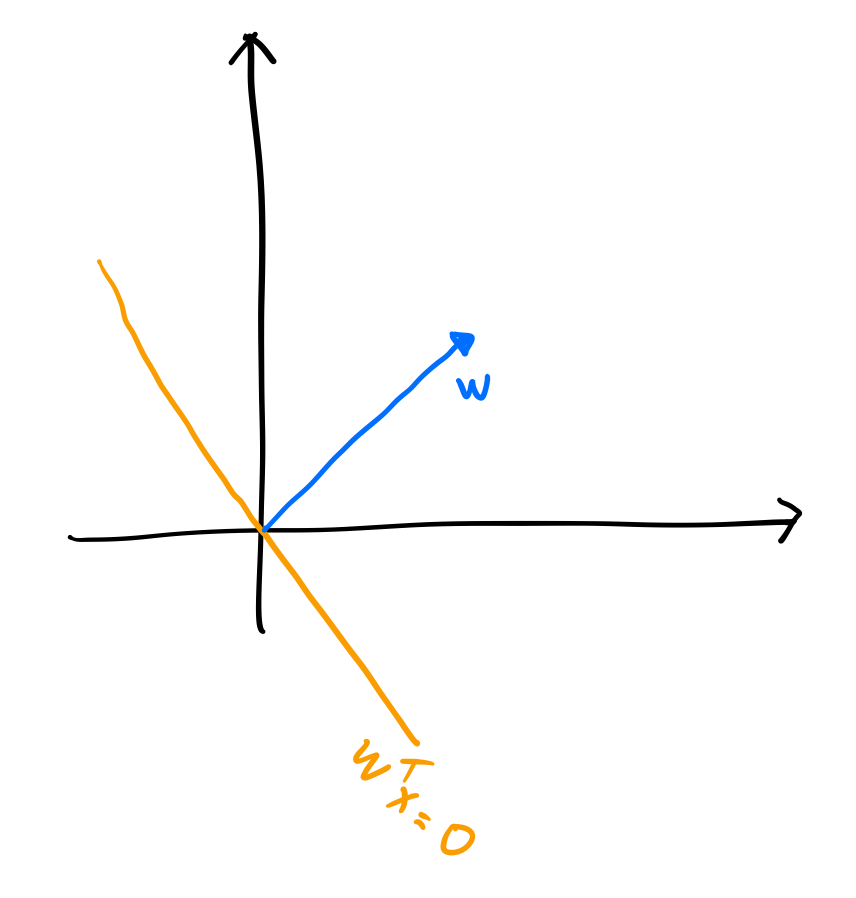
\includegraphics[scale=0.19]{./figs/SVM_Fig4.png} &\hspace{1cm}
	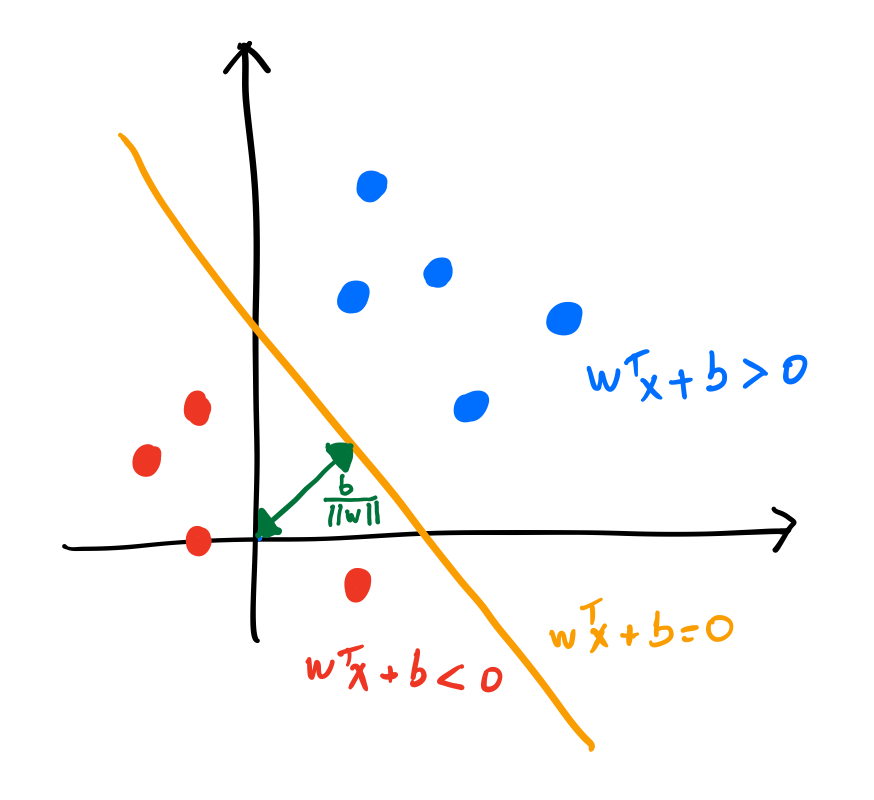
\includegraphics[scale=0.19]{./figs/SVM_Fig5.png}
\end{tabular}
\end{center}\vspace{-1cm}
}

\Sli{
\justify Definimos, também, como \textbf{hiplerplano canônico} $H$ aquele cujas amostras mais próximas satisfaçam $|\boldsymbol{w}^T\boldsymbol{x}+b|=1$. Como ilustrado abaixo, temos que os hiperplanos $H_1$ e $H_2$ definem, então, as margens com relação ao hiperplano canônico. 

\begin{center}
	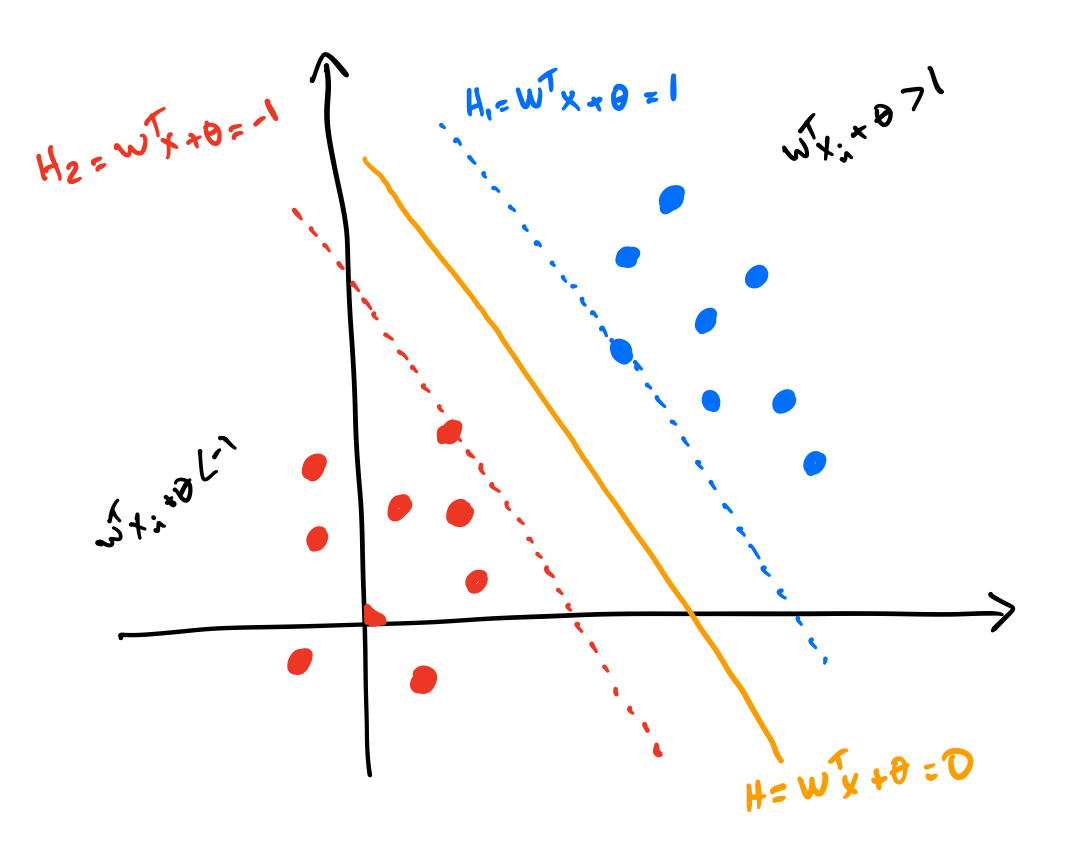
\includegraphics[scale=0.19]{./figs/SVM_Fig6.png}
\end{center}
}

\Sli{
\justify \underline{Definição do problema:} dado um conjunto de treinamento rotulado, isto é, classificação supervisionada, ${\cal X}^1=\{(\boldsymbol{x}_1,y_1),(\boldsymbol{x}_2,y_2),\ldots,(\boldsymbol{x}_m,y_m)\}$, as amostras mais próximas do hiperplano canônico $H$ devem satisfazer as seguintes condições:

\begin{itemize}
	\item $H_1:\boldsymbol{w}^T\boldsymbol{x}_i+b=1\implies \boldsymbol{w}^T\boldsymbol{x}_i+(b-1)=0$
	\item $H_2:\boldsymbol{w}^T\boldsymbol{x}_i+b=-1\implies \boldsymbol{w}^T\boldsymbol{x}_i+(b+1)=0$
\end{itemize}

\justify Em termos de classificação, temos que:

\begin{equation}\nonumber
	\boldsymbol{w}^T\boldsymbol{x}_i+b \leq -1\text{ se $y_i = -1$}
\end{equation}
e
\begin{equation}\nonumber
	\boldsymbol{w}^T\boldsymbol{x}_i+b \geq 1\text{ se $y_i = 1$}.
\end{equation}
}

\Sli{
Podemos unificar as equações anteriores da seguinte forma:

\begin{equation}
	y_i(\boldsymbol{w}^T\boldsymbol{x}_i+b)-1\geq 0,
\end{equation}
que é conhecida pela \textbf{restrição do problema}. 

\justify Note que teremos $m$ restrições, ou seja, uma para cada amostra do conjunto de treinamento, o que é bastante custoso para o classificador. Esse é um dos motivos que torna o SVM uma técnica bastante cara computacionalmente, sendo um dos seus principais pontos negativos.
}

\Sli{
Como podemos calcular a distância $d(H_1,h_2)$ entre os hiperplanos?

\begin{minipage}{0.43\textwidth}
\begin{center}
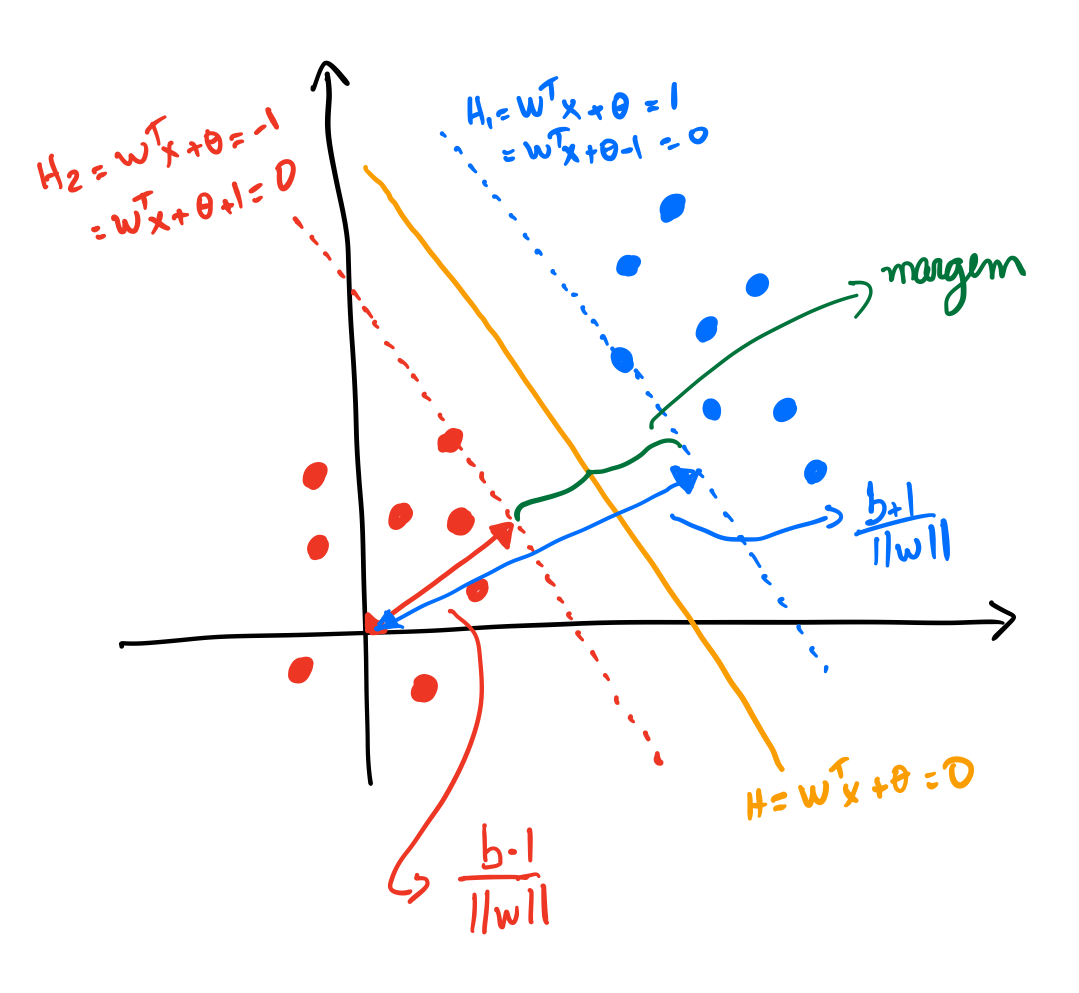
\includegraphics[scale=0.17]{./figs/SVM_Fig7.png}
\end{center}
\end{minipage}%%% to prevent a space
\begin{minipage}{0.49\textwidth}
\begin{align}\nonumber
	d(H_1,h_2) &= \frac{b+1}{\norm{\boldsymbol{w}}}-\frac{b-1}{\norm{\boldsymbol{w}}}\\
	&= \frac{(b+1)-(b-1)}{\norm{\boldsymbol{w}}}\\\nonumber
	&= \frac{b+1-b+1}{\norm{\boldsymbol{w}}}\\\nonumber
	&= \frac{2}{\norm{\boldsymbol{w}}}	\nonumber
\end{align}
\null
\par\xdef\tpd{\the\prevdepth}
\end{minipage}
}

\end{document}